% move all configuration stuff into one file so we can focus on the content
\documentclass[aspectratio=169,hyperref={pdfpagelabels=false,colorlinks=true,linkcolor=white,urlcolor=blue},t]{beamer}

%%%%%%%%%%%%%%%%%%%%%%%%%%%%%%%%%%%%%%%%%%%%%%%%%%%%%%%%%%%%%%%%%%%%%%%%%%%%%%%%%%
%%%%%%%%%%%%%%%%%%%%%%%%%%%%%%%%%%%%%%%%%%%%%%%%%%%%%%%%%%%%%%%%%%%%%%%%%%%%%%%%%%
% packages
\usepackage{pict2e}
\usepackage{epic}
\usepackage{amsmath,amsfonts,amssymb}
\usepackage{units}
\usepackage{fancybox}
\usepackage[absolute,overlay]{textpos} 
\usepackage{media9} % avi2flv: "C:\Program Files\ffmpeg\bin\ffmpeg.exe" -i TuneFreqFilterbank.avi -b 600k -s 441x324 -r 15 -acodec copy TuneFreqFilterbank.flv
\usepackage{animate}
\usepackage{gensymb}
\usepackage{multirow}
\usepackage{silence}
\usepackage[backend=bibtex,style=ieee]{biblatex}
\AtEveryCitekey{\iffootnote{\tiny}{}}
\addbibresource{references}

%%%%%%%%%%%%%%%%%%%%%%%%%%%%%%%%%%%%%%%%%%%%%%%%%%%%%%%%%%%%%%%%%%%%%%%%%%%%%%%%%%
%%%%%%%%%%%%%%%%%%%%%%%%%%%%%%%%%%%%%%%%%%%%%%%%%%%%%%%%%%%%%%%%%%%%%%%%%%%%%%%%%%
% relative paths
\graphicspath{{graph/}}


%%%%%%%%%%%%%%%%%%%%%%%%%%%%%%%%%%%%%%%%%%%%%%%%%%%%%%%%%%%%%%%%%%%%%%%%%%%%%%%%%%
%%%%%%%%%%%%%%%%%%%%%%%%%%%%%%%%%%%%%%%%%%%%%%%%%%%%%%%%%%%%%%%%%%%%%%%%%%%%%%%%%%
% units
\setlength{\unitlength}{1mm}

%%%%%%%%%%%%%%%%%%%%%%%%%%%%%%%%%%%%%%%%%%%%%%%%%%%%%%%%%%%%%%%%%%%%%%%%%%%%%%%%%%
%%%%%%%%%%%%%%%%%%%%%%%%%%%%%%%%%%%%%%%%%%%%%%%%%%%%%%%%%%%%%%%%%%%%%%%%%%%%%%%%%%
% theme & layout
\usetheme{Frankfurt}
\beamertemplatenavigationsymbolsempty
%\setbeamertemplate{frametitle}[smoothbars theme]
\setbeamertemplate{frametitle}
{
    \begin{beamercolorbox}[ht=1.8em,wd=\paperwidth]{frametitle}
        \vspace{-.1em}%
        \hspace{.2em}{\strut\insertframetitle\strut}
        
        \hspace{.2em}\small\strut\insertframesubtitle\strut
        %\hfill
        %
\includegraphics[height=.8cm,keepaspectratio]{CenterMusicTechnology-solid-2lines-white-CoAtag}
        
    \end{beamercolorbox}
    \begin{textblock*}{100mm}(11.6cm,.7cm)
        \includegraphics[height=.8cm,keepaspectratio]{logo_GTCMT_black}
    \end{textblock*}
}

% set this to ensure bulletpoints without subsections
\usepackage{remreset}
\makeatletter
\@removefromreset{subsection}{section}
\makeatother
\setcounter{subsection}{1}

%---------------------------------------------------------------------------------
% appearance
\setbeamercolor{structure}{fg=gtgold}
\setbeamercovered{transparent} %invisible
\setbeamercolor{bibliography entry author}{fg=black}
\setbeamercolor*{bibliography entry title}{fg=black}
\setbeamercolor*{bibliography entry note}{fg=black}

%\usepackage{pgfpages}
%\setbeameroption{show notes}
%\setbeameroption{show notes on second screen=right}
%---------------------------------------------------------------------------------
% fontsize
\let\Tiny=\tiny

%%%%%%%%%%%%%%%%%%%%%%%%%%%%%%%%%%%%%%%%%%%%%%%%%%%%%%%%%%%%%%%%%%%%%%%%%%%%%%%%%%
%%%%%%%%%%%%%%%%%%%%%%%%%%%%%%%%%%%%%%%%%%%%%%%%%%%%%%%%%%%%%%%%%%%%%%%%%%%%%%%%%%
% warnings
\pdfsuppresswarningpagegroup=1
\WarningFilter{biblatex}{Patching footnotes failed}
\WarningFilter{latexfont}{Font shape}
\WarningFilter{latexfont}{Some font shapes}
\WarningFilter{gensymb}{Not defining}



\subtitle{Part 6.6: Key and Chord Detection}

%%%%%%%%%%%%%%%%%%%%%%%%%%%%%%%%%%%%%%%%%%%%%%%%%%%%%%%%%%%%%%%%%%%%%%%%%%%%
\begin{document}
    % generate title page
	

\begin{frame}
    \titlepage
    %\vspace{-5mm}
    \begin{flushright}
        \href{http://www.gtcmt.gatech.edu}{\includegraphics[height=.8cm,keepaspectratio]{logo_GTCMT_black}}
    \end{flushright}
\end{frame}


    \section[overview]{lecture overview}
        \begin{frame}{key and chord detection}{overview}
            \begin{itemize}
                \item   \textbf{text book}  
                    \begin{itemize}
                        \item   \href{http://ieeexplore.ieee.org/xpl/articleDetails.jsp?tp=&arnumber=6331122&}{\underline{\textit{Chapter 5: Tonal Analysis} (pp.~108--117)}}
                    \end{itemize}
                \item   \textbf{sources}: slides (latex) \& Matlab  
                    \begin{itemize}
                        \item   \href{https://github.com/alexanderlerch/ACA-Slides}{\underline{github repository}}
                    \end{itemize}
                \bigskip
                \item<2->   \textbf{lecture content}
                    \begin{itemize}
                        \item<2->   pitch chroma representation
                        \item<3->   key detection
                        \item<4->   chord detection
                    \end{itemize}
            \end{itemize}
        \end{frame}

    \section[pitch chroma]{pitch chroma}
        \begin{frame}{pitch chroma}{introduction}
            \begin{itemize}
                \item	pitch class distribution
                \item	12-dimensional vector
            \end{itemize}
            \only<2->{\figwithmatlab{PitchChroma}}
            \only<3->{
            \begin{itemize}
                \item	\textbf{no} octave information
                    \begin{itemize}
                        \item	robust representation
                        \item	no differentiation between prime and octave
                    \end{itemize}
            \end{itemize}
            }                
        \end{frame}
        \begin{frame}{pitch chroma}{computation 1/2}
            \begin{enumerate}
                \item	divide spectral representation into \textbf{semi-tone bands}
                \item<2->	compute \textbf{mean per band}
                    \begin{footnotesize}
                        \begin{equation*}
                            \mu(j,n)		= \frac{1}{k_{\mathrm{u}}(j)-k_{\mathrm{l}}(j)+1}\sum\limits_{k=k_{\mathrm{l}}(j)}^{k_{\mathrm{u}}(j)}{|X(k,n)|}
                        \end{equation*}
                    \end{footnotesize}
                \item<3->	sum/mean every 12th band
                    \begin{footnotesize}
                        \begin{eqnarray*}
                            \nu(j\% 12 ,n)		&=& \sum\limits_{o=o_l}^{o_u}{\mu(j,n)}\label{eq:pc}, \\
                            \vec{\nu}(n) 	&=& \left[\nu(0,n),\, \nu(1,n),\, \nu(2,n),\, \ldots,\, \nu(10,n),\, \nu(11,n)\right]^\mathrm{T} \nonumber
                        \end{eqnarray*}
                    \end{footnotesize}
            \end{enumerate}
        \end{frame}
        \begin{frame}{pitch chroma}{computation 2/2}
            \figwithmatlab{PitchChromaGrouping}
        \end{frame}
        \begin{frame}{pitch chroma}{computation: variants}
            \begin{itemize}
                \item	\textbf{STFT}: 
                    \begin{itemize}
                        \item   \textit{weighted} mean of bins (window function)
                        \item	\textit{tonalness preprocessing}
                    \end{itemize}
                \item<2->	sum of \textbf{filterbank} output energies
                    \only<2>{\vspace{-5mm}\figwithmatlab{ResonanceFilterBank}}
                \item<3->	\textbf{CQT}: sum of bins/peaks
                \item<4->   beat-synchronous chroma
            \end{itemize}
        \end{frame}
        \begin{frame}{pitch chroma}{normalization}
            \begin{columns}[T]
                \column{.6\textwidth}
                    \begin{itemize}
                        \item   pitch chroma as \textit{distribution}:
                            \begin{equation*}
                                \sum\limits_{k=0}^{11}{\nu(k,n)} = 1
                            \end{equation*}
                        \item<2->   pitch chroma as \textit{vector}:
                            \begin{equation*}
                                \sqrt{\sum\limits_{k=0}^{11}{\nu(k,n)^2}} = 1
                            \end{equation*}
                        \item<3-> other options:
                            \begin{itemize}
                                \item   e.g., short-term energy normalization (CENS)
                            \end{itemize}
                    \end{itemize}
                \column{.4\textwidth}
                    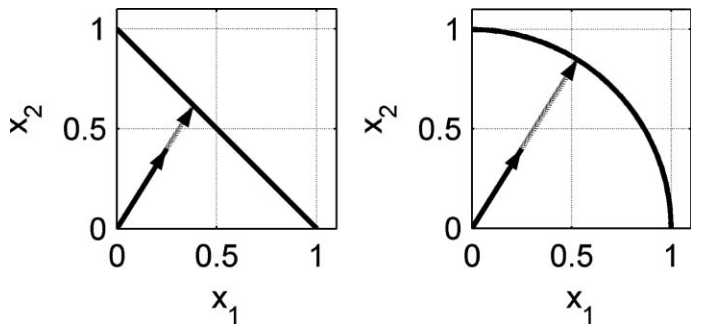
\includegraphics[scale=.2]{pc-norm}
            \end{columns}
            
        \end{frame}
        
        \begin{frame}{pitch chroma}{problems 1/2}
            %usual assumption: pitch chroma contains only \textit{fundamental frequency components}
            
            \figwithmatlab{HarmonicsInPitchChroma}
            \begin{itemize}
                \item	\textbf{problem 1}: amplitude distortion due to harmonics
                        \begin{itemize}
                            \item<2->	[$\Rightarrow$]	de-emphasize higher frequencies
                            \item<3->	[$\Rightarrow$]	build amplitude model
                            \item<4->	[$\Rightarrow$]	use multi-pitch detection system
                        \end{itemize}
            \end{itemize}
        \end{frame}
        \begin{frame}{pitch chroma}{problems 2/2}
            \begin{itemize}
                \item	\textbf{problem 2}: frequency distortion due to Harmonics
                \begin{table}
                    \centering
                    \begin{tabular}{cccccccccccc} %{\textwidth}{@{\extracolsep{\fill}}ccccccccccccc}
                        \\ \hline
                        \bf{\emph{Harmonic}}	 & \bf{\emph{$|\Delta C(f,f_T)|$}}\\ 
                         \hline
                        \bf{$f = f_0$}	 & 0\\
                        \bf{$f = 2\cdot f_0$}	 & 0\\
                        \bf{$f = 3\cdot f_0$}	 & 1.955\\
                        \bf{$f = 4\cdot f_0$}	 & 0\\
                        \bf{$f = 5\cdot f_0$}	 & 13.6863\\
                        \bf{$f = 6\cdot f_0$}	 & 1.955\\
                        \bf{$f = 7\cdot f_0$}	 & 31.1741\\
                        \hline
                        \bf{$\mu_{|\Delta C|}$}	 & 6.9672\\
                    \end{tabular}
                \end{table}
            \end{itemize}
        \end{frame}

    \section{key detection}
        \begin{frame}{key detection}{brainstorm}
            \question{what are your ideas for detecting the key in a complex mixture}
        \end{frame}
        \begin{frame}{key detection}{introduction 1/2}
        \only<1>{
            assumptions: pitch class distribution is prototypical for key
            \begin{itemize}
                \item	tonic/root note is tonal center
                \item	tonal and harmonic relations define importance and occurrence of individual pitch classes
            \end{itemize}
            }
        \end{frame}
        \begin{frame}{key detection}{introduction 2/2}
            \begin{enumerate}
                \item<1->	define reference distribution for specific keys
                    \only<1>{\figwithmatlab{KrumhanslKeyProfile}}
                \item<2->	extract average pitch chroma
                \item<3->	compute distance between template and extracted chroma
                    \only<3>{            
                    \begin{figure}
                        \begin{center}
                        \begin{picture}(60,25)
                
                            %boxes
                            \put(0,10){\ovalbox{\footnotesize{\parbox{20mm}{\centering{extracted\\ pitch chroma}}}}}
                            \put(0,20){\ovalbox{\footnotesize{\parbox{20mm}{\centering{template\\ pitch chroma}}}}}
                            \put(27,15){\ovalbox{\footnotesize{\parbox{20mm}{\centering{distance measure}}}}}
                
                        
                            %diagonal
                            \put(22.5,11){\vector(1,1){4.5}}
                            \put(22.5,21){\vector(1,-1){4.5}}
                            
                            % horizontal
                            \put(49,15.5){\vector(1,0){10}}
                
                            %text
                            \put(54,16){\footnotesize{\shortstack[c]{key}}}
                
                        \end{picture}
                        \end{center}
                    \end{figure}
                    }
                    \only<4>{\videowithmatlab{KeyDetection}}

            \end{enumerate}
        \end{frame}
        
        \begin{frame}{key detection}{key templates 1/2}
                    \begin{itemize}
                        \item	\emph{Orthogonal} $\vec{\nu}_\mathrm{o}$: root note is most salient component, other components negligible
                                \pause
                                \begin{itemize}
                                    \item	same distance to all keys
                                    \item	no distinction between major and minor
                                \end{itemize}
                        \item<2->	\emph{Smoothed Orthogonal} $\vec{\nu}_\mathrm{s}$:  root note most salient, neighboring components less important
                                \pause
                                \begin{itemize}
                                    \item	increasing key distance to tritone
                                    \item	no real distinction between major and minor
                                \end{itemize}
                        \item<3->	\emph{Diatonic} $\vec{\nu}_\mathrm{d}$: all key-inherent pitches weighted equally
                                \pause
                                \begin{itemize}
                                    \item	linear increasing key distance
                                \end{itemize}
                        \item<4->	\emph{Probe tone Ratings}  $\vec{\nu}_\mathrm{p}$: derived from perceptual tonal similarity
                        \item<5->	\emph{Extracted Key Profiles} $\vec{\nu}_\mathrm{t}$: derived from real-world data
                    \end{itemize}
        \end{frame}
        \begin{frame}{key detection}{key templates 2/2}
            \figwithmatlab{KeyProfiles}
        \end{frame}
        \begin{frame}{key detection}{distance measures: (vector) distance}
            \begin{footnotesize}
                    \begin{itemize}
                        \item	\emph{{Euclidean distance}}:
                                $d_\mathrm{E}(s) = \sqrt{\sum\limits_{j = 0}^{11}{\big(\nu_\mathrm{e}(j)-\nu_\mathrm{t,s}(j)\big)^2}} $
                        \item<2->	\emph{{Manhattan distance}}:
                                $d_\mathrm{M}(s) = \sum\limits_{j = 0}^{11}{\big|\nu_\mathrm{e}(j)-\nu_\mathrm{t,s}(j)\big|} $
                        \item<3->	\emph{{Cosine distance}}:
                                $d_\mathrm{C}(s) = 1-\left( \frac{\sum\limits_{j = 0}^{11}{\nu_\mathrm{e}(j)\cdot\nu_\mathrm{t,s}(j)}}{\sqrt{\sum\limits_{j = 0}^{11}{\nu_\mathrm{e}(j)^2}}\sqrt{\cdot \sum\limits_{j = 0}^{11}{\nu_\mathrm{t,s}(j)^2}}}\right) $
                        \item<4->	\emph{{Kullback-Leibler divergence}}:
                                $d_\mathrm{KL}(s) = \sum\limits_{j = 0}^{11}{\nu_\mathrm{e}(j)\cdot\log\left(\frac{\nu_\mathrm{e}(j)}{\nu_\mathrm{t,s}(j)}\right)}$
                        \item<5->   \textit{nearest neighbor classification}
                    \end{itemize}
            \end{footnotesize}
        \end{frame}
        %%\begin{frame}{key detection}{distance measures: k-Nearest Neighbor}
            %%\begin{itemize}
                %%\item	\textbf{training}: extract reference vectors from training set (keep class labels)
                %%\pause
                %%\item	\textbf{classification}: extract test vector and set class to majority of $k$ nearest reference vectors
            %%\end{itemize}
                %%\begin{figure}[t]
                    %%\centering
                        %%\includegraphics[scale=.7]{graph/KnnClassification}
                %%\end{figure}
        %%\end{frame}
        \begin{frame}{key detection}{variants}
            \begin{itemize}
                \item	\textbf{tonalness weight}:\\ estimate the tonality/noisiness and weight instantaneous pitch chroma
                \item<2->	\textbf{multiple estimations}:\\ split piece into regions and estimate key through majority
                \item<3->	\textbf{real-time key detection}:\\ estimate in sliding window
            \end{itemize}
        \end{frame}
        \begin{frame}{key detection}{results \& typical errors}
            \begin{columns}[T]
            \column{.6\textwidth}
                \begin{itemize}
                    \item	typical errors: related keys
                        \begin{itemize}
                            \item	Dominant
                            \item	Subdominant
                            \item	Relative
                            \item	Major/Minor
                        \end{itemize}
                \end{itemize}
            \column{.4\textwidth}
                \begin{figure}
                    \centering
                        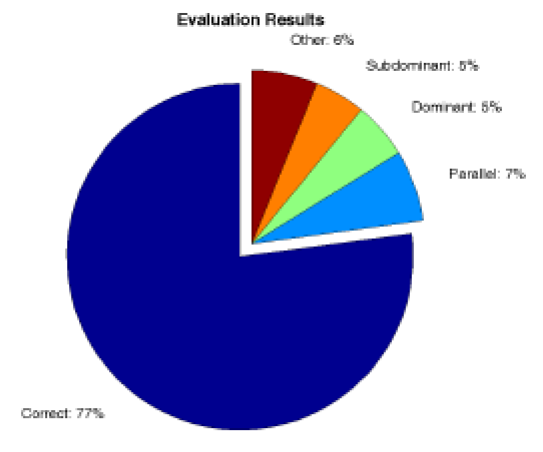
\includegraphics[scale=.35]{resultskeydetection}
                \end{figure}
            \end{columns}
            \begin{flushright}
                graph from \footfullcite{lerch_ansatz_2004}
            \end{flushright}
        \end{frame}

    \section{chord detection}
        \begin{frame}{chord detection}{brainstorm}
           \question{what are your ideas for detecting the chords in a complex mixture}
        \end{frame}
        \begin{frame}{chord detection}{introduction}
            \question{discuss commonalities and differences between chord \& key detection}

            \begin{itemize}
                \item	\textbf{commonalities}
                    \begin{itemize}
                        \item<2->	chords are octave independent $\Rightarrow$ pitch chroma sufficient
                        \item<2->	process flow: pitch chroma extraction $+$ classification
                    \end{itemize}
                \item<3->	\textbf{differences}
                    \begin{itemize}
                        \item	time frame for pitch chroma calculation
                        \item	templates
                        \item	number of templates/chords
                        \item	many results per song (time series)
                    \end{itemize}
            \end{itemize}
        \end{frame}
        \begin{frame}{chord detection}{chord template}
            \begin{itemize}
                \item	linear transformation template: 
            
                    example: major $[\nicefrac{1}{3},0,0,0,\nicefrac{1}{3},0,0,\nicefrac{1}{3},0,0,0,0]$
                \item	instantaneous chord likelihood:
                \begin{equation*}
                    {\psi}(0,n) = \sum\limits_{j = 0}^{11}{\Gamma(0,j)\cdot \nu(j,n)}
                \end{equation*}
            \end{itemize}	
        \end{frame}
        
        \begin{frame}{chord detection}{chord progression 1/2}
            apply \textbf{musical knowledge} to increase the result's robustness and accuracy:
            
            \begin{itemize}
                \item	different probabilities for different chord progressions (similar to key modulations), e.g.
                \begin{itemize}
                    \item	cadences: I-IV-V-I
                    \item	sequences: circle progression
                    
                \end{itemize}
            \end{itemize}

            $\Rightarrow$ model for \textit{chord progression probabilities}
            \begin{itemize}
                \item<2->	\textit{analytical model} based on music theory
                    \begin{itemize}
                        \item	circle of fifths (?!)
                        \item	key profile correlation (?!)
                    \end{itemize}
                \item<3->	\textit{empirical model} based on data
                    \begin{itemize}	
                        \item	annotate audio
                        \item	symbolic score
                    \end{itemize}
            \end{itemize}
        \end{frame}
        \begin{frame}{chord detection}{chord progression 2/2}
            \question{what properties do chord progression probabilities depend on}

            \begin{itemize}
                \item 	musical key
                \item<3->	larger musical context (model order)
                \item<4->	style
            \end{itemize}
        \end{frame}
        
        \begin{frame}{chord detection}{markov chain}
            \begin{figure}
                \centering
                    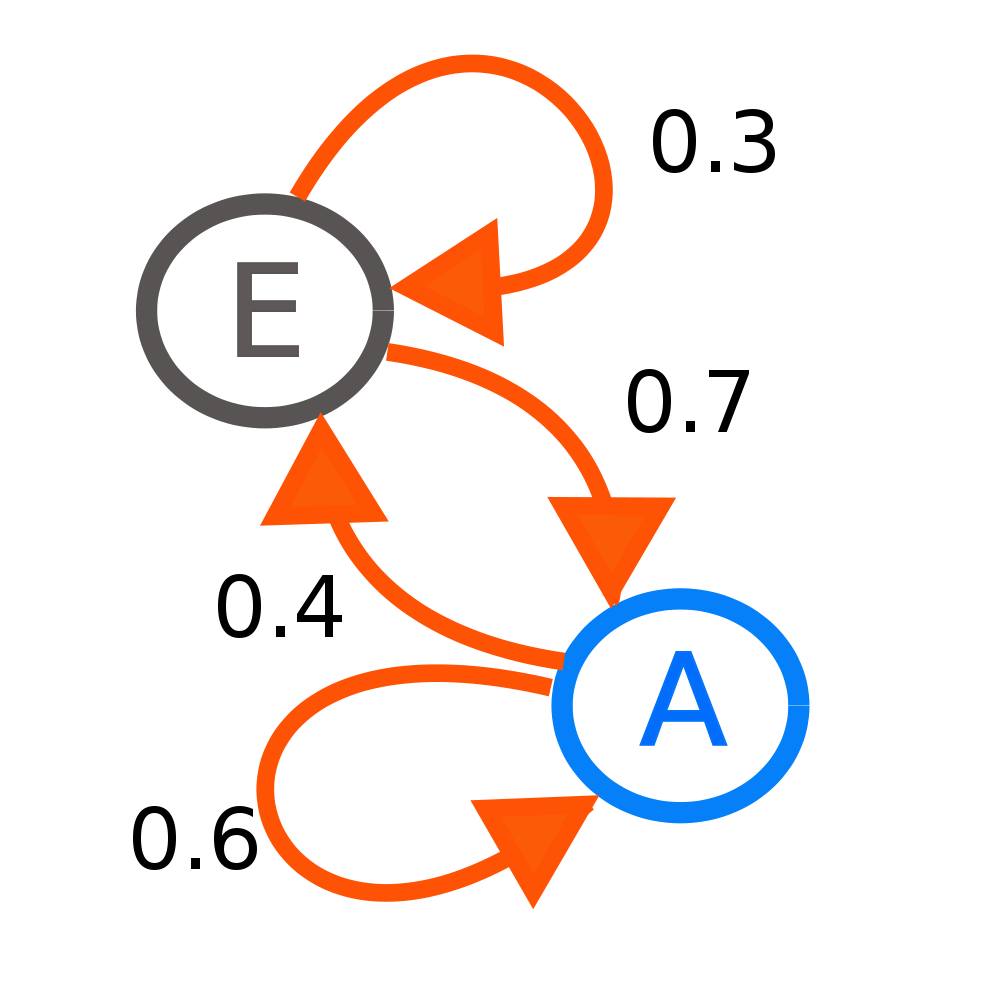
\includegraphics[scale=.1]{graph/MarkovChain}
            \end{figure}
            \addreference{from: \url{https://commons.wikimedia.org/wiki/File:Markovkate_01.svg}}
            \begin{itemize}
                \item   two possible states E, A
                \item   transition probabilities to other state(s) and to self
                \item   sum of transition probabilities equals 1
            \end{itemize}
        \end{frame}
        
        \begin{frame}{chord detection}{hidden markov model: variables}
            \begin{itemize}
                \item	\textbf{states}:\\ unknown/hidden
                \smallskip
                \item	\textbf{transition probability}:\\ probability of transitioning from one state to the other
                \smallskip
                \item   \textbf{observations}:\\ measureable time series
                \smallskip
                \item	\textbf{emission probability}:\\ probability of a state given an observation
                \smallskip
                \item	\textbf{start probability}:\\ probability of the initial state
            \end{itemize}
        \end{frame}
        \begin{frame}{chord detection}{hidden markov model: variables}
            \begin{figure}[t]
                \centering
                    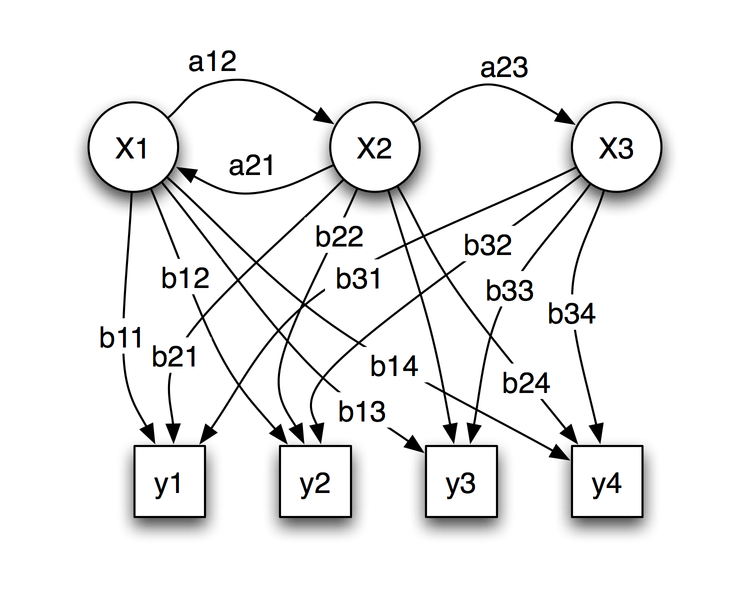
\includegraphics[scale=.25]{graph/HiddenMarkovModel}
            \end{figure}
            \addreference{from \url{https://en.wikipedia.org/wiki/File:HiddenMarkovModel.svg}}
            \vspace{-5mm}
            \begin{footnotesize}
                \begin{itemize}
                    \item	X: states
                    \item	y: possible observations
                    \item	a: state transition probabilities
                    \item	b: emission probabilities
                \end{itemize}
            \end{footnotesize}
        \end{frame}
        \begin{frame}{chord detection}{hidden markov model: example (WP) 1/2}
            \begin{itemize}
                \item   \textbf{scenario}
                    \begin{itemize}
                        \item   doctor diagnoses fever by how patients feel
                        \item   patient may feel normal, dizzy, or cold
                        \item   patient visits multiple days in a row 
                    \end{itemize}
            \end{itemize}
            \question{what are the states and observations in this case}
            
            \begin{itemize}
                \item	\textbf{states} %: \textit{healthy}, \textit{fever}
                    \begin{itemize}
                        \item   \textit{healthy}
                        \item   \textit{fever}
                    \end{itemize}
                \item   \textbf{observations}: %\textit{normal}, \textit{cold}, \textit{dizzy}
                    \begin{itemize}
                        \item   \textit{normal}
                        \item   \textit{cold}
                        \item   \textit{dizzy}
                    \end{itemize}
            \end{itemize}
        \end{frame}
        \begin{frame}{chord detection}{hidden markov model: example (WP) 2/2}
            \begin{columns}[T]
            \column{.6\textwidth}
            \begin{itemize}
                \item   \textbf{start probabilities} (initial state assumption)
                    \begin{itemize}
                        \item   \textit{healthy}: $ 0.6$
                        \item   \textit{fever}: $0.4$
                    \end{itemize}
                \item<2->   \textbf{emission probabilities} (prob of obs given state)
                    \begin{itemize}
                        \item   \textit{healthy}: normal $0.5$, cold $0.4$, dizzy $0.1$
                        \item   \textit{fever}: : normal $0.1$, cold $0.3$, dizzy $0.6$
                    \end{itemize}
                \item<3->   \textbf{transition probabilities}
                    \begin{itemize}
                        \item   \textit{healthy}: healthy $0.7$, fever $0.3$
                        \item   \textit{fever}: : healthy $0.4$, fever $0.6$
                    \end{itemize}
            \end{itemize}
            \column{.4\textwidth}
            \only<4->{
                    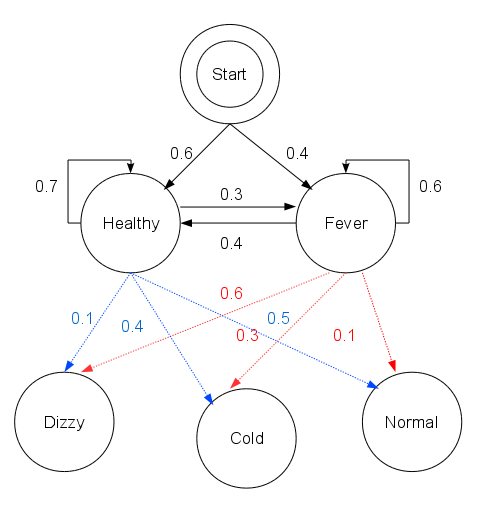
\includegraphics[scale=.35]{HmmExample}
            }
            \end{columns}
            \addreference{from: \url{https://en.wikipedia.org/wiki/File:An_example_of_HMM.png}}
        \end{frame}
        \begin{frame}{chord detection}{hidden markov model: example (WP) 2/2}

            \begin{itemize}
                \item<5->   \textbf{three observations}:\\ \textit{normal} $\rightarrow$ \textit{cold} $\rightarrow$ \textit{dizzy}
            \end{itemize}
            \setcounter{i}{0}
            \whiledo{\value{i}<5}	
            {
                \only<\value{beamerpauses}>
                {
                    \begin{figure}
                    \centering
                        \includegraphics[scale=.8]{graph/viterbi_\arabic{i}}
                    \end{figure}
                }
                \ifthenelse{\equal{\value{i}}{4}}{}{\pause}
                \stepcounter{i} 
            }	
            \visible<1->{\addreference{from: \url{https://en.wikipedia.org/wiki/Viterbi_algorithm\#/media/File:Viterbi_animated_demo.gif}}}
        \end{frame}
        \begin{frame}{chord detection}{HMMs for chord detection}
            \begin{itemize}
                \item   states $\rightarrow$ chords
                \item   observations $\rightarrow$ pitch chroma
                \item   emission probability $\rightarrow$ trained with pitch chroma
                \item   transition probability $\rightarrow$ trained from dataset
                \item   start probability $\rightarrow$ chord statistics
            \end{itemize}
        \end{frame}
        
        \section[summary]{lecture summary}
        \begin{frame}{summary}{lecture content}
            \begin{enumerate}
                \item   discuss advantages and disadvantages of the pitch chroma representation
                \smallskip
                \item<2->   what are typical variants in calculating the pitch chroma
                \smallskip
                \item<3->   describe the processing block of a simple key detection system
                \smallskip
                \item<4->   in what aspects are key and chord detection similar and dissimilar
                \smallskip
                \item<5->   discuss the advantages and disadvantages of using an HMM for chord detection
            \end{enumerate}
        \end{frame}
\end{document}

